\chapter[Literature Review]{Literature Review}
\label{Chap:Literature}


% ***************************************************
% Literature Review
% ***************************************************

% ********* Enter your text below this line: ********

\section{Heading 1}
%Replace "Heading 1" with what will become the \label{} for this section.
\begin{itemize}
	\item On the subject of determining the historical nature of past sources and sources (ontology)
	\item Identifying past sources (epistemology)
	\item Look critically at past sources.
	\item Showing the difference between your work and past work
\item	Comparing the results of your work with past work
	\item Pointing out weaknesses in past work and demonstrating the reasons for conducting the research
\end{itemize}
\subsection{Heading 2}
\lipsum[4] % This generates dummy text to fill the document


\begin{table}[h]
    \begin{tabular}{|>{\bfseries}p{0.25\linewidth} | p{0.30\linewidth} | p{0.35\linewidth}|}
        \hline
        Column 1 &  \textbf{Column 2} &  \textbf{Column 3}\\ 
        \hline
        Lorem Ipsum   & Dolor sit amet    & Consectetur adipiscing\\ 
        \hline
        Vivamus luctus& Tempor incididunt & Magna aliqua\\ 
        \hline
        Ut enim ad    & Minim veniam      & Quis nostrud exercitation\\ 
        \hline
    \end{tabular}
    \caption{Lorem Ipsum}
    \label{tab:2-1}
\end{table}


\begin{figure}[h]
\begin{center}
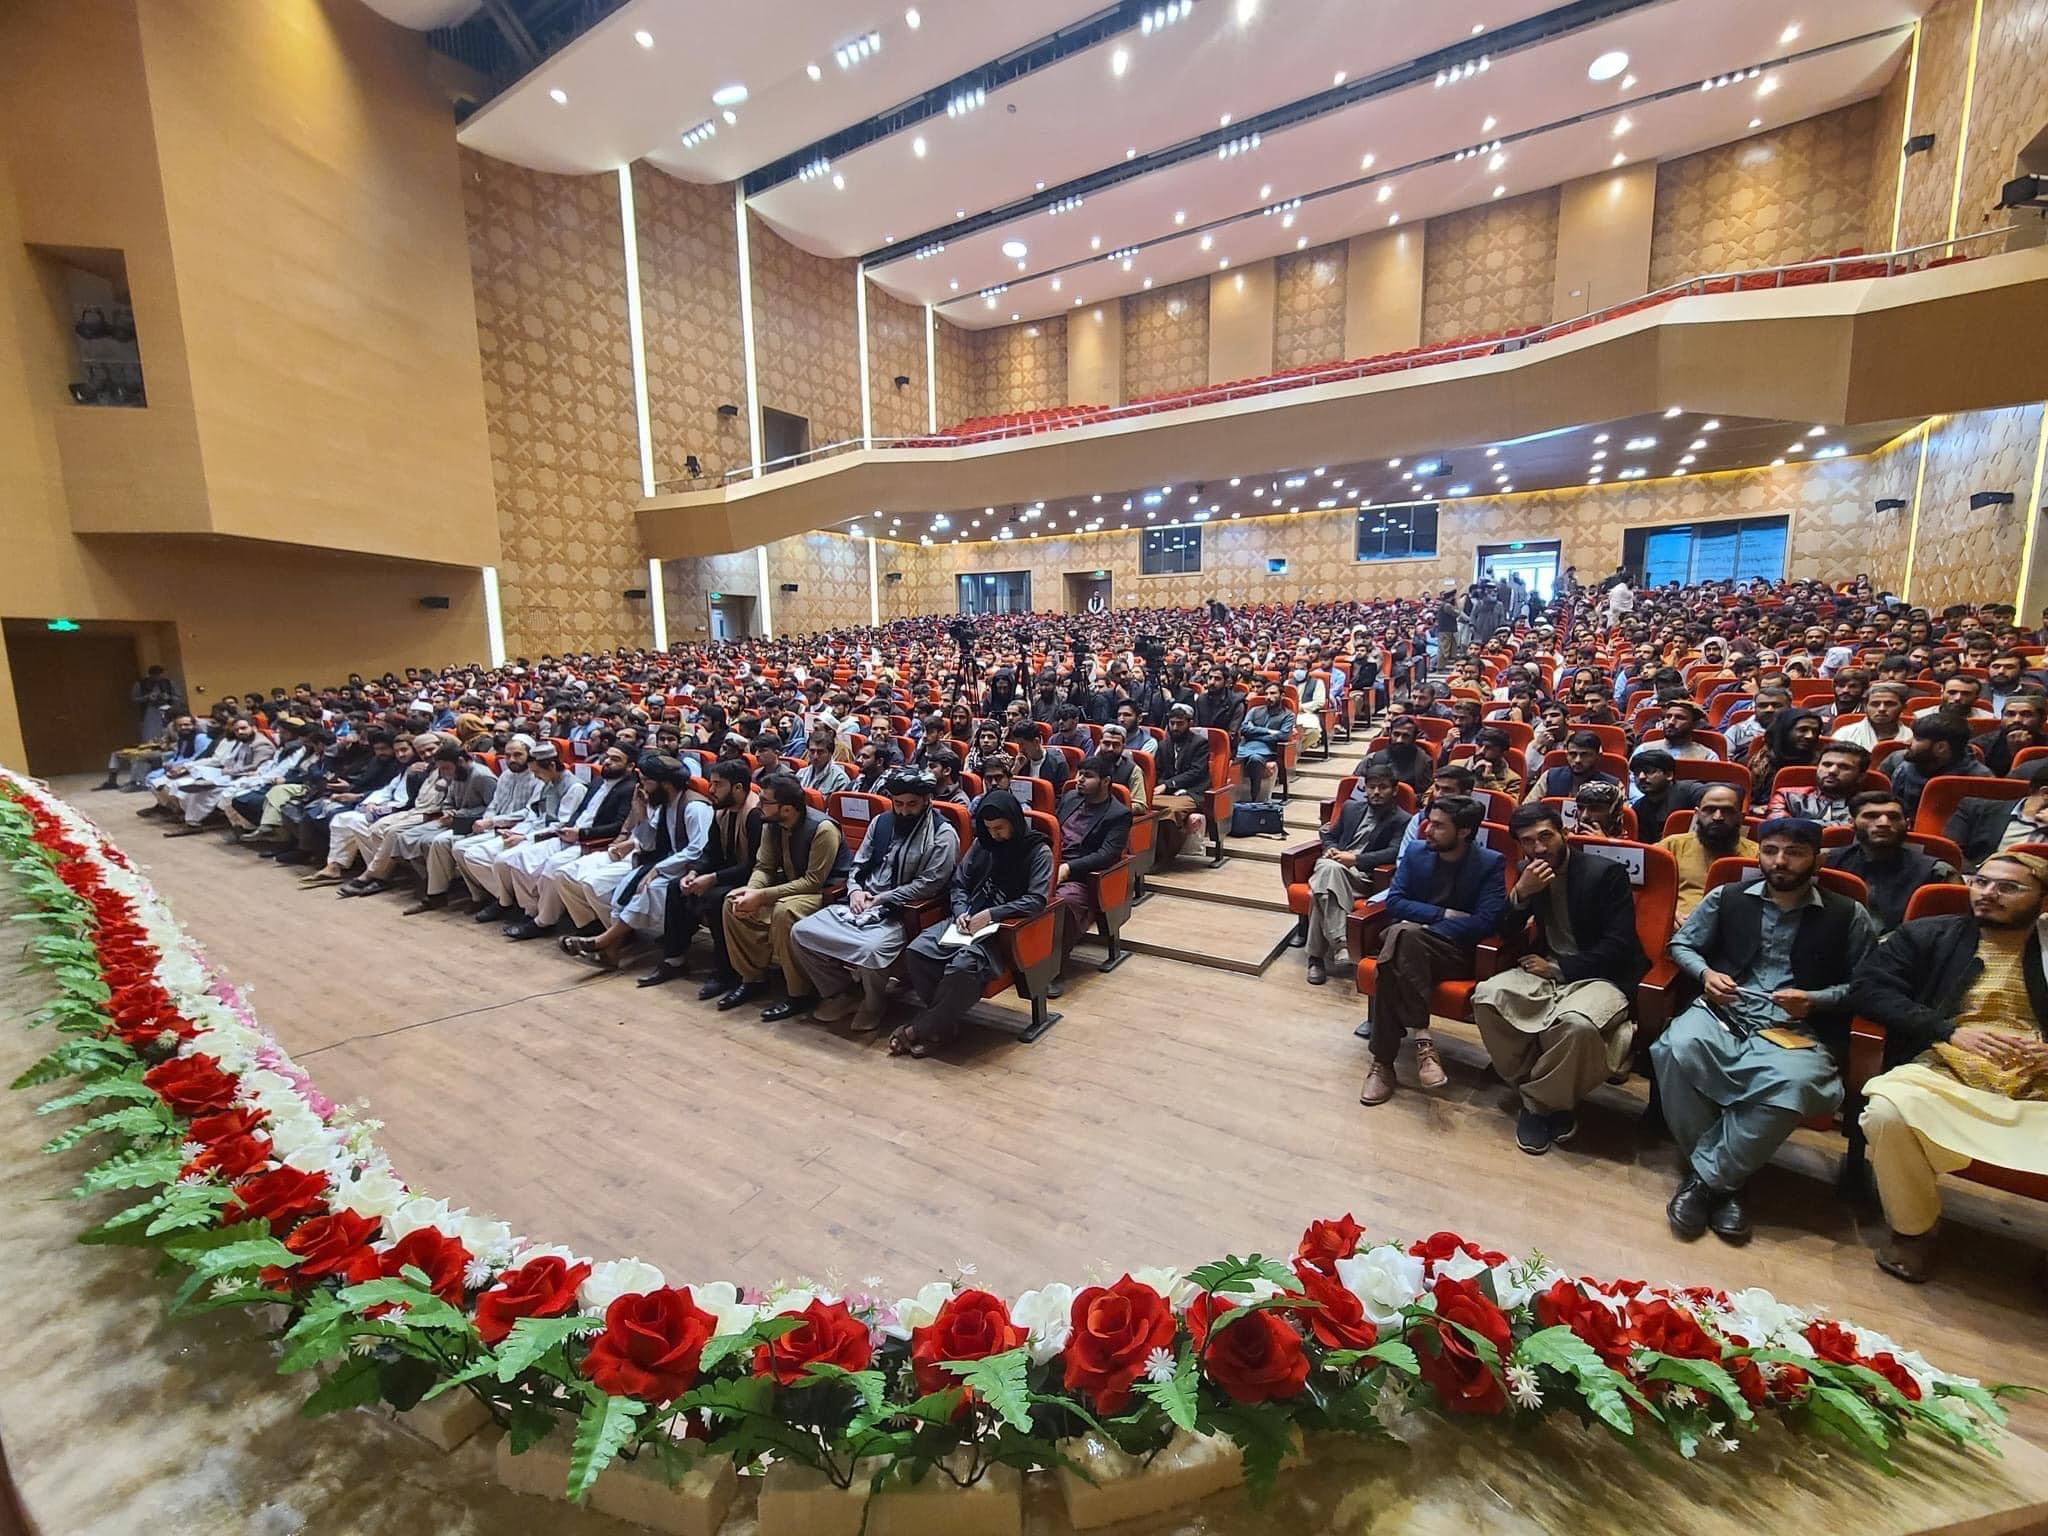
\includegraphics[width=1.0\textwidth]{Resources/KU2}
\caption{Kabul University}
\label{Figure:Kabul University}
\end{center}
\end{figure}

% ***************************************************